\documentclass{jsarticle}
\bibliographystyle{ipsjunsrt.bst}
\usepackage[dvipdfmx]{graphicx, xcolor, hyperref}
\usepackage{amsmath}
\usepackage{spverbatim}
\usepackage{bm}%太字ベクトル
\hypersetup{
    colorlinks=true,
    citecolor=blue,
    linkcolor=gray,
    urlcolor=blue
}
\title{レポート課題3:補間,数値積分}
\author{工学研究科M1 1030340103 三角聡}
\date{\today}

\makeatletter
\newcommand{\verbatimfont}[1]{\renewcommand{\verbatim@font}{\ttfamily#1}}
\makeatother

\begin{document}
\maketitle
以下の課題について数値計算の演習を行う.今回はコードなどの提出は必要ありません.
レポートは課題の結果をグラフで示し,簡単な考察を書くこと.

\section{補間 Interpolation}
次の関数$f(x)$に対して区間$[-1,1]$で,
\begin{enumerate}
\item チェビシェフ点を用いた8次多項式補間
\item 3次自然スプライン補間(8区間)
\end{enumerate}
のそれぞれを求め,元の関数値とグラフ上で比較せよ.
$$f(x)=\frac{1}{1+36x^2}$$

図\ref{interpolation-fig}に元の関数,チェビシェフ点を用いた8次多項式補間,スプライン補間を重ねて示す.
8次多項式補間では区間分割が無く一つの多項式で近似しているため,全てのxで全次数$f^{(0)}~f^{(8)}$が連続であるが,その連続性の制約が強く働き補間点以外では振動し近似が正確ではない.一方,三次スプライン補間は区間を分割し$f'''$が不連続であることを許容しているので$f,f',f''$を元の関数に近づける自由度が確保されており,比較的正確な補間ができている.


\begin{figure}[htbp]
    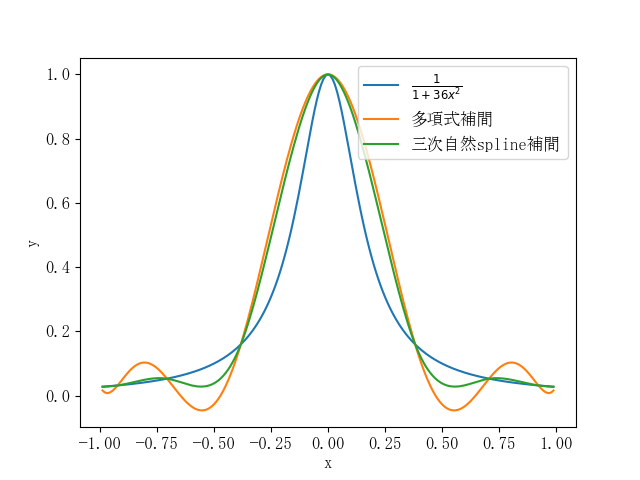
\includegraphics[keepaspectratio, width=16cm]{figures/interpolation.pdf}
  \centering
  \caption{補間手法の比較\label{interpolation-fig}}
\end{figure}

\section{数値積分 Numerical integral}

次の定積分$I(f)$に対して次に示す各手法で数値積分を行い,真の解に対する誤差を議論せよ.
\begin{enumerate}
\item ロンバーグ積分 Romberg integration
\\初期の区間数 Initial partition:$n=1$
\\繰り返し回数  Iteration: $J=3$
\\つまり,$T_{8n}^{(3)}$まで計算してください.ということです.Means, calculate until $T_{8n}^{(3)}$.
\item 3次自然スプライン補間(8区間)
\\クレンショー・カーチス則 Crenshaw Curtis rule
\\8次補間 (8th order interpolation)
\end{enumerate}

$$I(f)=\int_0^2 e^x dx$$

図\ref{integration-fig}に各数値積分手法の比較を示す.$\int_0^2 e^x$の積分においてromberg積分は相対誤差$4.54\times10^{-8}$と実用上十分な精度が出ている一方でCrenshaw-Curtis則では相対誤差$2.08\times 10^{-2}$で精度が比較的に低いと言える.被積分関数の評価回数は両者とも8回だが,romberg積分が等間隔に被積分関数を評価するのに対し,Crenshaw-Curtis則ではチェビシェフ多項式を用いて中央より区間端を重点的に評価している点が精度に影響を与えていると考えられる.ただし,Crenshaww-Curtis則の計算に誤りがある可能性は否定できない.

\begin{figure}[htbp]
    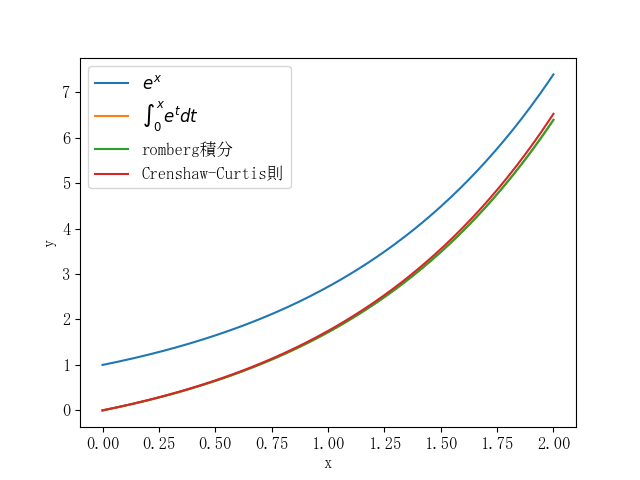
\includegraphics[keepaspectratio, width=16cm]{figures/integration.pdf}
  \centering
  \caption{数値積分手法の比較\label{integration-fig}}
\end{figure}

\section{ソースコード}

pythonで記述した.実行には外部ライブラリとしてmatplotlibが必要である.

\pagebreak
\begin{spverbatim}
import math, numpy
import matplotlib.pyplot as plt


def make_figure():
    plt.rcParams['font.family'] = 'MS Mincho'
    plt.rcParams["font.size"] = 12
    fig = plt.figure()
    ax = fig.add_subplot(111)
    return fig, ax


def interpolation_function(x):  # 補間元の関数
    return 1 / (1 + 36 * x ** 2)


def integration_function(x):  # 積分元の関数
    return math.exp(x)


def get_chebyshev_point(a, b, k):  # チェビシェフ補間点の配列を返す関数
    return [(b - a) / 2 * math.cos(math.pi * j / k) + (b + a) / 2 for j in range(0, k + 1)]


def get_polynomial_interpolation_function(f, x, n):  # 多項式補間した関数fを返す関数
    print("多項式補間", "N={}".format(n))
    if len(x) != n + 1:
        raise ValueError("次数と補間点数の不一致")
    y = [f(v) for v in x]
    x_matrix = [[v ** i for i in range(0, n + 1)] for v in x]
    a = numpy.linalg.solve(x_matrix, y)
    return lambda xa: sum(a[i] * xa ** i for i in range(0, n + 1))


def get_cubic_natural_spline(f, x):  # 多項式補間した関数fを返す関数
    N = len(x) - 1  # x_0 x_1 ... x_N
    print("3次自然スプライン補間", "N={}".format(N))
    y = [f(x_i) for x_i in x]
    d = y
    h = [x[i + 1] - x[i] for i in range(0, N)]
    w = [6 * ((y[i + 1] - y[i]) / h[i] - (y[i] - y[i - 1]) / h[i - 1]) if i >= 1 else 0 for i in range(0, N)]
    A = numpy.identity(N - 1)
    for i in range(N - 1):
        A[i][i] = 2 * (h[i] + h[i + 1])
        if i != N - 2:
            A[i][i + 1] = h[i + 1]
        if i != 0:
            A[i][i - 1] = h[i]
    v = numpy.linalg.solve(A, w[1:N])
    v = numpy.insert(numpy.insert(v, 0, 0), N, 0)
    b = v / 2
    a = [(v[i + 1] - v[i]) / (6 * (x[i + 1] - x[i])) for i in range(0, N)]
    c = [(y[i + 1] - y[i]) / (x[i + 1] - x[i]) - (x[i + 1] - x[i]) * (2 * v[i] + v[i + 1]) / 6 for i in range(N)]
    return lambda xa: sum(
        a[i] * (xa - x[i]) ** 3 + b[i] * (xa - x[i]) ** 2 + c[i] * (xa - x[i]) + d[i]
        if (x[i] - xa) * (x[i + 1] - xa) < 0 else 0
        for i in range(N)
    )


def romberg_integration(func, a, b, init_n=1, iteration=3): # ロンバーグ積分を行う関数
    # 複合中点則
    M = lambda f, n: (b - a) / n * sum(f(a + (b - a) / n * (k + 0.5)) for k in range(n))
    # 複合台形則
    T = lambda f, n: (b - a) / n * ((f(a) + f(b)) / 2 + sum(f(a + (b - a) / n * (k + 1)) for k in range(n - 1)))
    T_array = []
    for i in range(iteration + 1):
        if i != 0:
            pass

        if False:  # T(0)の決定法はどちらでもよい
            T_0 = T(func, init_n * 2 ** i)
        else:
            if i == 0:
                T_0 = T(func, init_n)
            else:
                T_0 = (T_array[0] + M(func, init_n * 2 ** (i - 1))) / 2
        T_array_new = [T_0]
        for j in range(1, 1 + i):
            T_array_new.append((T_array[j - 1] - 2 ** (2 * j) * T_array_new[-1]) / (1 - 2 ** (2 * j)))
        T_array = T_array_new
    return T_array[-1]


def crenshaw_curtis_integration(func, a, b, n):
    f = lambda t: (b - a) / 2 * func((b + a) / 2 + (b - a) / 2 * t)
    # a_0~a_n:
    a = [
        2 / n * sum(f(math.cos(math.pi / n * i)) * math.cos(math.pi / n * j * i) for i in range(n + 1))
        for j in range(n + 1)
    ]
    # print(a)
    l_max = int((n + 1) / 2)
    return sum(2 * a[2 * l] / (1 - 4 * l ** 2) * (1 if 0 < l < l_max else 0.5) for l in range(0, l_max + 1))


if __name__ == '__main__':
    print("補間")
    points = get_chebyshev_point(-1, 1, 8)
    print("チェビシェフ点", points)
    x = [i / 100 for i in range(-99, 100)]
    fig, ax = make_figure()
    ax.plot(x, [interpolation_function(i) for i in x], label=r'$\frac{1}{1+36x^2}$')
    fp = get_polynomial_interpolation_function(interpolation_function, points, 8)
    ax.plot(x, [fp(i) for i in x], label="多項式補間")
    fs = get_cubic_natural_spline(interpolation_function, points)
    ax.plot(x, [fs(i) for i in x], label="三次自然spline補間")
    ax.set_xlabel("x")
    ax.set_ylabel("y")
    ax.legend()
    fig.savefig("interpolation.pdf")
    print("数値積分")
    fig, ax = make_figure()
    x=[i/100 for i in range(0,201)]
    ax.plot(x, [integration_function(i) for i in x], label="$e^x$")
    correct_value = [math.exp(i)-1 for i in x]
    ax.plot(x, correct_value, label="$\int_0^x e^t dt$")
    print("真値", x[-1], correct_value[-1])
    value = [romberg_integration(integration_function, 0, i, iteration=3) for i in x]
    ax.plot(x, value, label="romberg積分")
    print("romberg積分", "積分=", value[-1], "相対誤差=", abs((value[-1] - correct_value[-1]) / correct_value[-1]))
    value = [crenshaw_curtis_integration(integration_function, 0, i, 8) for i in x]
    ax.plot(x, value, label="Crenshaw-Curtis則")
    print("Crenshaw-Curtis則", "積分=", value[-1], "相対誤差=", abs((value[-1] - correct_value[-1]) / correct_value[-1]))
    ax.set_xlabel("x")
    ax.set_ylabel("y")
    ax.legend()
    fig.savefig("integration.pdf")
    plt.show()

\end{spverbatim}

実行結果を以下に示す.グラフとして図\ref{interpolation-fig}のinterpolation.pdfと図\ref{integration-fig}のintegration.pdfが出力される.

\begin{spverbatim}
補間
チェビシェフ点 [1.0, 0.9238795325112867, 0.7071067811865476, 0.38268343236508984, 6.123233995736766e-17, -0.3826834323650897, -0.7071067811865475, -0.9238795325112867, -1.0]
多項式補間 N=8
3次自然スプライン補間 N=8
数値積分
真値 2.0 6.38905609893065
romberg積分 積分= 6.389056389097693 相対誤差= 4.541626147912277e-08
Crenshaw-Curtis則 積分= 6.522215719492969 相対誤差= 0.02084182991985406
\end{spverbatim}


\end{document}